%%%%%%%%%%%%%%%%%%%%%%%%%%%%%%%%%%%%%%%%%%%%%%
% Head matter - can we try to be consistent on
% included packages
\ifdefined\beamerclass
\else
    \def\beamerclass{beamer}
\fi
\documentclass[\beamerclass]{beamer}

\usepackage{pgfpages}
\usepackage{pgfplots}
\mode<handout>{
  % \setbeamercolor{background canvas}{bg=black!20}
  \pgfpagesuselayout{2 on 1}[a4paper,border shrink=5mm]
}

%\documentclass{beamer}
\mode<presentation>
{\usetheme{default}
 \usecolortheme{default}
 \usefonttheme{default}
 \setbeamertemplate{navigation symbols}{}
 \setbeamertemplate{footline}[frame number]
% \setbeamertemplate{caption}[numbered]
 }
\usepackage[english]{babel}
\usepackage{algorithm}
\usepackage[noend]{algpseudocode}
\usepackage[utf8x]{inputenc}
\usepackage{graphicx}
\usepackage{hyperref}
%\graphicspath{{./images/}}
\usepackage{tikz}
\usetikzlibrary{shapes.geometric, arrows,chains}
\usepackage{booktabs,makecell,multirow,tabularx}
\usepackage{verbatim}
\renewcommand{\arraystretch}{1.2}
\renewcommand\theadfont{\normalfont\bfseries}
\usepackage{array}
\usepackage{listings}
\lstset{language=Java, showstringspaces=false}
\usepackage[normalem]{ulem}
\usepackage{bm}
\def\layersep{2.5cm}

\usepackage{xcolor}
%\usepackage{subfig}
\setbeamertemplate{caption}{\insertcaption}
\usepackage[caption=false]{subfig}
\usepackage{hyperref}
\usepackage{verbatim}
%\setbeamertemplate{caption}[numbered]%\numberwithin{figure}{section}
% Define block styles

\usetheme{Copenhagen}
\hypersetup{pdfstartview={Fit}}
\lstset{basicstyle=\small\ttfamily,breaklines=true}

\usepackage{xmpmulti}
%\setbeamertemplate{caption}[numbered]%\numberwithin{figure}{section}
% Define block styles
\tikzstyle{decision} = [diamond, draw, fill=blue!20, 
    text width=4.5em, text badly centered, node distance=3cm, inner sep=0pt]
\tikzstyle{block} = [rectangle, draw, fill=blue!20, 
    text width=3em, text centered, rounded corners, minimum height=3em]
\tikzstyle{line} = [draw, -latex']
\tikzstyle{cloud} = [draw, ellipse, fill=red!20, node distance=3cm,
    minimum height=2em]
\tikzset{
  startstop/.style={
    rectangle, 
    rounded corners,
    minimum width=3cm, 
    minimum height=1cm,
    align=center, 
    draw=black, 
    fill=red!30
    },
  process/.style={
    rectangle, 
    minimum width=3cm, 
    minimum height=1cm, 
    align=center, 
    draw=black, 
    fill=blue!30
    },
  decision/.style={
    rectangle, 
    minimum width=3cm, 
    minimum height=1cm, align=center, 
    draw=black, 
    fill=green!30
    },
  arrow/.style={thick,->,>=stealth},
  dec/.style={
    ellipse, 
    align=center, 
    draw=black, 
    fill=green!30
    },
}
\tikzstyle{arrow} = [thick,->,>=stealth]

\tikzset{onslide/.code args={<#1>#2}{%
  \only<#1>{\pgfkeysalso{#2}} % \pgfkeysalso doesn't change the path
}}

\makeatletter
\newenvironment<>{btHighlight}[1][]
{\begin{onlyenv}#2\begingroup\tikzset{bt@Highlight@par/.style={#1}}\begin{lrbox}{\@tempboxa}}
{\end{lrbox}\bt@HL@box[bt@Highlight@par]{\@tempboxa}\endgroup\end{onlyenv}}

\newcommand<>\btHL[1][]{%
  \only#2{\begin{btHighlight}[#1]\bgroup\aftergroup\bt@HL@endenv}%
}
\def\bt@HL@endenv{%
  \end{btHighlight}%   
  \egroup
}
\newcommand{\bt@HL@box}[2][]{%
  \tikz[#1]{%
    \pgfpathrectangle{\pgfpoint{1pt}{0pt}}{\pgfpoint{\wd #2}{\ht #2}}%
    \pgfusepath{use as bounding box}%
    \node[anchor=base west, fill=orange!30,outer sep=0pt,inner xsep=1pt, inner ysep=0pt, rounded corners=3pt, minimum height=\ht\strutbox+1pt,#1]{\raisebox{1pt}{\strut}\strut\usebox{#2}};
  }%
}
\makeatother

\definecolor{darkblue}{RGB}{37,55,97}
\definecolor{mellowyellow}{RGB}{247,206,70}
\definecolor{almostwhite}{RGB}{254,255,255}
\definecolor{merrygreen}{RGB}{79,173,91}
\definecolor{funkyorange}{RGB}{240,154,56}

\addtobeamertemplate{footnote}{\hskip -2em}{}
\newcommand\blfootnote[1]{%
  \begingroup
  \renewcommand\thefootnote{}\footnote{#1}%
  \addtocounter{footnote}{-1}%
  \endgroup
}

\DeclareMathOperator{\softmax}{softmax}
\DeclareMathOperator{\softplus}{softplus}
\DeclareMathOperator{\ReLU}{ReLU}
\DeclareMathOperator{\argmax}{arg\,max}
\DeclareMathOperator{\abs}{abs}
\DeclareMathOperator{\huber}{huber}

\AtBeginSection[]{
  \begin{frame}
  \vfill
  \centering
  \begin{beamercolorbox}[sep=8pt,center,shadow=false,rounded=true]{title}
    \usebeamerfont{title}\insertsectionhead\par%
  \end{beamercolorbox}
  \vfill
  \end{frame}
}

%%%%%%%%%%%%%%%%%%%%%%%%%%%%%%%%%%%%%%%%%%%%%%
% Formatting for title page
\title[Generative Models]{Deep Generative Modelling}
\author{Jonathon Hare}
\institute[]
{
  Vision, Learning and Control\\
  University of Southampton 
}
\date{}
\subject{Computer Science}
\useoutertheme{infolines}
\setbeamertemplate{headline}{} %remove headline
\setbeamertemplate{navigation symbols}{} %remove navigation symbols
%%%%%%%%%%%%%%%%%%%%%%%%%%%%%%%%%%%%%%%%%%%%%%

\begin{document}

\begin{frame}[plain]
        \begin{tikzpicture}[overlay, remember picture, shift={(current page.south west)},font={\fontfamily{Montserrat-TOsF}\selectfont}]
        \fill [darkblue,text=almostwhite] (0,0) rectangle (\paperwidth, \paperheight);
        \draw (4,7) node [align=left,text=almostwhite] {\Huge 
        \begin{tabular}{l} 
        \textbf{Yes,}\\
        \textbf{we GAN.}
        \end{tabular}};
        \draw (11,1) node [align=left,text=almostwhite] {\includegraphics[scale=0.15]{../vlc.png}};
        \end{tikzpicture}
\end{frame}

\begin{frame}
  \titlepage
\end{frame}

%-------------------------------------------------------------%
%\begin{frame}[fragile]{pause}\frametitle{Deep Autoencoder}
%\begin{center}
%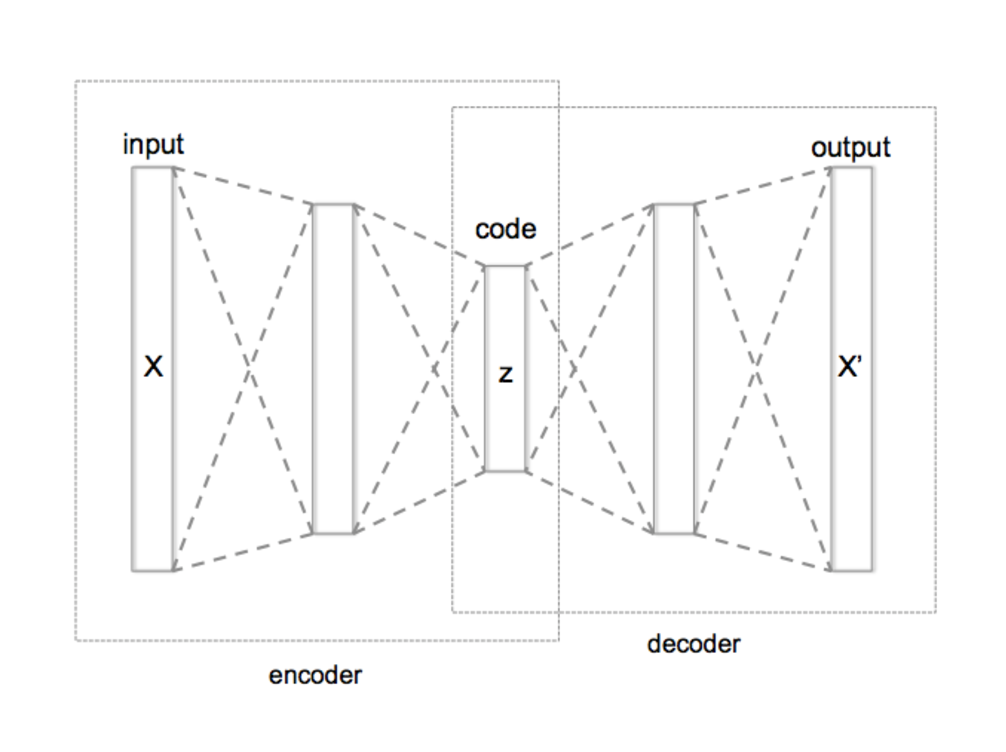
\includegraphics[width=10cm]{DAE.pdf} \footnote{Image taken from wikipedia}
%\end{center}
%\end{frame}
%-------------------------------------------------------------%
\begin{frame}\frametitle{Introduction}
\begin{itemize}
\item What is generative modelling and why do we do it?
\item Differentiable Generator Networks
\item Variational Autoencoders
\item Generative Adversarial Networks
\end{itemize}
\end{frame}

%-------------------------------------------------------------%

\section{Generative Modelling and Differentiable Generator Networks}
\begin{frame}\frametitle{Recap: Generative Models}
\begin{itemize}
  \item<1-> Learn models of the data: $p(\mathrm{x})$ 
  \item<1-> Learn \emph{conditional} models of the data: $p(\mathrm{x}|\mathrm{y}=y)$
  \item<+-> Some generative models allow the probability distributions to be evaluated explicitly
  \begin{itemize}
    \item i.e. compute the probability of a piece of data $x$: $p(\mathrm{x}=x)$
  \end{itemize}
  \item<+-> Some generative models allow the probability distributions to be sampled
  \begin{itemize}
    \item i.e. draw a sample $x$ based on the distribution: $x \sim p(\mathrm{x})$
  \end{itemize}
  \item<+-> Some generative models can do both of the above
  \begin{itemize}
    \item<+-> e.g. a Gaussian Mixture Model is an explicit model of the data using $k$ Gaussians
    \begin{itemize}
      \item<+-> The likelihood of data $x$ is the weighted sum of the likelihood from each of the $k$ Gaussians
      \item<+-> Sampling can be achieved by sampling the categorical distribution of $k$ weights followed by sampling a data point from the corresponding Gaussian
    \end{itemize}
  \end{itemize}
\end{itemize}
\end{frame}

%-------------------------------------------------------------%

\begin{frame}\frametitle{Why do generative modelling?}
\begin{itemize}
  \item<+-> Try to understand the processes through which the data was itself generated
  \begin{itemize}
    \item Probabilistic latent variable models like VAEs or topic models (PLSA, LDA, \dots) for text
    \item Models that try to disentangle latent factors like $\beta$-VAE
  \end{itemize}
  \item<+-> Understand how likely a new or previously unseen piece of data is
  \begin{itemize}
    \item outlier prediction, anomaly detection, \dots
  \end{itemize}
  \item<+-> Make `new' data
  \begin{itemize}
    \item Make `fake' data to use to train large supervised models?
    \item `Imagine' new, but plausible, things?
  \end{itemize}
\end{itemize}
\end{frame}

%-------------------------------------------------------------%

\begin{frame}\frametitle{Differentiable Generator Networks}
\begin{itemize}
  \item<+-> Generative Modelling is not new; we've known how to make arbitrarily complex probabilistic graphical models for many years.
  \begin{itemize}
    \item ...But difficult to train and scale to real data, relying on MCMC.
  \end{itemize}
  \item<+-> The past few years has seen major progress along four loose strands:
  \begin{itemize}
    \item<+-> Invertible density estimation - A way to specify complex generative models by transforming a simple latent distribution with a series of invertible functions. 
    \item<+-> Autoregressive models - Another way to model $p(x)$ is to break the model into a series of conditional distributions: $p(x)=p(x_1)p(x_2|x_1)p(x_3|x_2,x_1)\dots$
    \item<+-> Variational autoencoders - Latent-variable models that use a neural network to do approximate inference.
    \item<+-> Generative adversarial networks - A way to train generative models by optimizing them to fool a classifier
  \end{itemize}
  \item<+-> \textbf{Common thread in recent advances is that the loss functions are end-to-end differentiable.}
\end{itemize}
\end{frame}

%-------------------------------------------------------------%

\begin{frame}\frametitle{Differentiable Generator Networks: key idea}
\begin{itemize}
  \item We're interested in models that transform samples of latent variables $\bm z$ to 
  \begin{itemize}
    \item samples $x$, or,
    \item distributions over samples $x$
  \end{itemize}
  \item The model is a (differentiable) function $g(\bm z, \bm\theta)$
  \begin{itemize}
    \item typically $g$ is a neural network.
  \end{itemize}
\end{itemize}

\end{frame}

%-------------------------------------------------------------%

\begin{frame}
\frametitle{Example: drawing samples from $\mathcal{N}(\bm\mu,\bm\Sigma)$}

\begin{itemize}
  \item<+-> Consider a simple generator network with a single affine layer that maps samples $\mathcal{N}(\bm 0,\bm I)$ to $\mathcal{N}(\bm\mu,\bm\Sigma)$: \\[1em]

  \begin{center}
  \begin{tikzpicture}[
            > = stealth, % arrow head style
            shorten > = 1pt, % don't touch arrow head to node
            auto,
            node distance = 3cm, % distance between nodes
            semithick % line style
        ]

         \node (i) {$\bm z \sim \mathcal{N}(\bm 0, \bm I)$};
         \node[draw = black,thick] (g) [right of=i] {$g_{\bm\theta}(\bm z)$};
         \node (o) [right of=g] {$\bm x \sim \mathcal{N}(\bm \mu, \bm \Sigma)$};
    
         \path[->] (i) edge node {} (g);
         \path[->] (g) edge node {} (o);
  \end{tikzpicture}
  \end{center}
  \item<+-> Note: Exact solution is $\bm x = g_{\bm\theta}(\bm z) = \bm\mu + \bm L \bm z$ where $\bm L$ is the Cholesky decomposition of $\bm\Sigma$: $\bm\Sigma = \bm L \bm L^\top$, lower triangular $\bm L$.
\end{itemize}


\end{frame}

%-------------------------------------------------------------%

\begin{frame}
\frametitle{Generating samples}

More generally, we can think of $g$ as providing a nonlinear change of variables that transforms a distribution over $\mathbf{z}$ into the desired distribution over $\mathbf{x}$:

\begin{center}
  \begin{tikzpicture}[
            > = stealth, % arrow head style
            shorten > = 1pt, % don't touch arrow head to node
            auto,
            node distance = 3cm, % distance between nodes
            semithick % line style
        ]

         \node (i) {$p_z(\bm z)$};
         \node[draw = black,thick] (g) [right of=i] {$g(\bm z)$};
         \node (o) [right of=g] {$p_x(\bm x)$};
    
         \path[->] (i) edge node {} (g);
         \path[->] (g) edge node {} (o);
  \end{tikzpicture}
\end{center}
\pause
  For any \emph{invertible, differentiable, continuous} $g$:

  \begin{equation*}
    p_z(\bm z) = p_x(g(\bm z)) \left| \det\left(\frac{\partial g}{\partial \bm z}\right)\right|
  \end{equation*}

  Which implicitly imposes a probability distribution over $\mathbf x$:

  \begin{equation*}
    p_x(\bm x) = \frac{p_z(g^{-1}(\bm x))}{\left| \det\left(\frac{\partial g}{\partial \bm z}\right)\right|}
  \end{equation*}
\pause
Note: usually use an indirect means of learning $g$ rather than minimise $-\log(p(\bm x))$ directly
\end{frame}

%-------------------------------------------------------------%

\begin{frame}
\frametitle{Generating distributions}
\begin{itemize}
  \item<+-> Rather than use $g$ to provide a sample of $\bm x$ directly, we could instead use $g$ to define a conditional distribution over $x$, $p(\bm x | \bm z)$
  \begin{itemize}
    \item For example, $g$ might produce the parameters of a particular distribution - e.g.:
    \begin{itemize}
      \item means of Bernoulli
      \item mean and variance of a Gaussian
    \end{itemize}
  \end{itemize}
  \item<+-> The distribution over $\bm x$ is imposed by marginalising $\bm z$:$ p(\bm x) = \mathbb{E}_{\bm z} p(\bm x | \bm z)$
\end{itemize}
\end{frame}

%-------------------------------------------------------------%

\begin{frame}
\frametitle{Distributions vs Samples}
\begin{itemize}
  \item<+-> In both cases ($g$ generates samples and $g$ generates distributions) we can use the reparameterisation tricks we saw last lecture to train models.
  \item<+-> Generating distributions:
  \begin{itemize}
     \item + works for both continuous and discrete data
     \item - need to specify the form of the output distribution
   \end{itemize} 
  \item<+-> Generating samples:
  \begin{itemize}
    \item + works for continuous data
    \begin{itemize}
      \item + discrete data is recently possible - we need the $\operatorname{STargmax}$
    \end{itemize}
    \item + don't need to specify the distribution in explicit form
  \end{itemize}

\end{itemize}
\end{frame}

%-------------------------------------------------------------%

\begin{frame}
\frametitle{Complexity of Generative Modelling}

\begin{itemize}
  \item<+-> In classification both input and output are given
  \begin{itemize}
    \item Optimisation only needs to learn the mapping
  \end{itemize}
  \item<+-> Generative modelling is more complex than classification because
  \begin{itemize}
    \item<+-> learning requires optimizing intractable criteria
    \item<+-> data does not specify both input $\bm z$ and output $\bm x$ of the generator network
    \item<+-> learning procedure needs to determine how to arrange $\bm z$ space in a useful way and how to map $\bm z$ to $\bm x$
  \end{itemize}
\end{itemize}
\end{frame}

%-------------------------------------------------------------%
\section{Variational Autoencoders}

\begin{frame}\frametitle{Variational Autoencoders (VAEs)}

The Variational Autoencoder uses the following generative process to draw samples:
\begin{center}
  \begin{tikzpicture}[
            > = stealth, % arrow head style
            shorten > = 1pt, % don't touch arrow head to node
            auto,
            node distance = 4.5cm, % distance between nodes
            semithick % line style
        ]

         \node (i) {$\bm z \sim p_{\mathrm{model}}(\bm z)$};
         \node[draw = black,thick] (g) [right of=i] {$p_{\mathrm{model}}(\bm x | \bm z; \bm\theta) = p_{\mathrm{model}}(\bm x; g_{\bm\theta}(\bm z))$};
         \node (o) [right of=g] {$\bm x \sim p_{\mathrm{model}}(\bm x | \bm z; \bm\theta)$};
    
         \path[->] (i) edge node {} (g);
         \path[->] (g) edge node {} (o);
  \end{tikzpicture}
  \begin{itemize}
    \item The learning problem is to find $\bm\theta$ that maximises the probability of each $\bm x$ in the training set under $p(\bm x) = \int\! p(\bm x | \bm z; \bm\theta) p(\bm z) d \bm z$
    \item $p_{\mathrm{model}}(\bm z)$ is most often chosen to be $\mathcal{N}(\bm 0, \bm I)$
    \item $p_{\mathrm{model}}(\bm x | \bm z)$ is chosen according to the data; typically Gaussian for real-valued data (most often just predicting the means, with a fixed diagonal covariance) or Bernoulli for binary data.
    \begin{itemize}
      \item Intuition: we don't exactly want to exactly create the training examples; we want to create things \emph{like} the training examples
    \end{itemize}
  \end{itemize}
\end{center}

\end{frame}

%-------------------------------------------------------------%

\begin{frame}\frametitle{Variational Autoencoders (VAEs)}
\begin{itemize}
  \item<+-> Conceptually we can compute $p(\bm x) \approx \frac{1}{n}\sum_i^n p(\bm x | \bm z_i; \bm\theta)$ for $n$ samples of $\bm z$, $\{\bm z_1, \dots, \bm z_n\}$ and just use gradient ascent to do the optimisation
  \begin{itemize}
    \item<+-> This isn't tractable in practice; $n$ would need to be \emph{extremely} big!
  \end{itemize}
  \item<+-> For most $\bm z$, $p(\bm x| \bm z)$ will be nearly zero, and hence contribute almost nothing to our estimate of $p(\bm x)$
  \item<+-> The key idea behind the VAE is to learn to sample values of $\bm z$ that are likely to have produced $\bm x$, and compute $p(\bm x)$ just from those
  \begin{itemize}
    \item<+-> Introduce a new function $q_{\bm\phi}(\bm z | \bm x)$ which can take a value of $\bm x$ and produce the distribution over $\bm z$ values that are likely to produce $\bm x$. 
    \item<+-> The space of $\bm z$ values that are likely under $q$ should be much smaller than the space of than under prior $p(\bm z)$.
    \item<+-> We can now compute $\mathbb{E}_{\bm z \sim q_{\bm\phi}} p(\bm x | \bm z; \bm \theta)$ easily
    \begin{itemize}
      \item if the PDF $q(\bm z)$, is not $\mathcal{N}(\bm 0, \bm I)$, then how does that help us optimize $p(\bm x)$?
      \item and how does this expectation relate to $p(\bm x)$?
    \end{itemize}
  \end{itemize}
\end{itemize}
\end{frame}

%-------------------------------------------------------------%
\begin{frame}
\frametitle{Variational Inference}
\begin{align*}
\onslide<1->{\text{\footnotesize Log-probability} && \log p(x) &= \log \int\! p(x|z) p(z) dz \\}
\onslide<2->{\text{\footnotesize Proposal} && \log p(x) &= \log \int\! p(x|z) p(z) \frac{q(z|x)}{q(z|x)} dz \\}
\onslide<3->{\text{\footnotesize Importance weight} && \log p(x) &= \log \int\! p(x|z) \frac{p(z)}{q(z|x)} q(z|x) dz \\}
\onslide<4->{\text{\footnotesize Jensen's inequality} && \log p(x) &\geq \int\! q(z|x) \log \left( p(x|z) \frac{p(z)}{q(z|x)} \right) dz \\}
\onslide<5->{\text{\footnotesize Rearrange} && \log p(x) &\geq \int\! q(z|x) \log p(x|z) dz - \int\! q(z|x) \log \frac{q(z|x)}{p(z)} dz \\}
\onslide<6->{\text{\footnotesize ELBO} && \log p(x) &\geq \mathbb{E}_{z\sim q(z|x)}\log p(x|z) - D_\mathrm{KL}(q(z|x)||p(z))}
\end{align*}

\scriptsize{
Jensen's inequality: $\log \int\! p(x) g(x) dx \geq \int\! p(x) \log g(x) dx$\\
Log product rule: $\log(a \cdot b)=\log a + \log b$\\
Log quotient rule: $\log(a / b)=\log a - \log b$
}
\end{frame}

%-------------------------------------------------------------%

\begin{frame}
\frametitle{The Evidence LOwer Bound (ELBO) / variational lower bound}

The ELBO expression we just derived is a cornerstone of variational inference:
\begin{align*}
  \mathcal{L}(q) &= \mathbb{E}_{\bm z \sim q(\bm z | \bm x)} \log p_\mathrm{model} (\bm x | \bm z) - D_\mathrm{KL}(q(\bm z |\bm x) || p_\mathrm{model}(\bm z)) \\
  &\leq \log p_\mathrm{model}(\bm x)
\end{align*}
\begin{itemize}
  \item The expectation term looks just like a reconstruction log-likelihood found in normal autoencoders
  \begin{itemize}
    \item If $p_{\mathrm{model}}(\bm x | \bm z)$ is Gaussian, then this is MSE between the true training $\bm x$ and a generated sample computed from $\bm z$, averaged across many $\bm z$'s (each a function of $\bm x$)
  \end{itemize}
  \item The KL term is forcing the approximate posterior $q(\bm z |\bm x)$ towards the prior $p_\mathrm{model}(\bm z)$.
\end{itemize}
\end{frame}

%-------------------------------------------------------------%

\begin{frame}
\frametitle{Why is it called an autoencoder?}

\begin{itemize}
  \item<+-> $q(\bm z |\bm x)$ is referred to as an encoder; it's used to take $\bm x$ and turn it into a $\bm z$
  \item<+-> $p_{\mathrm{model}}(\bm x; g_{\bm\theta}(\bm z))$ is referred to as a decoder network; it takes a $\bm z$ and decodes it into a target $\bm x$
  \item<+-> From a practical standpoint, a VAE is a normal autoencoder with two key differences:
  \begin{itemize}
    \item the encoder generates a distribution that must be sampled
    \begin{itemize}
      \item the network produces the sufficient statistics of the distribution (e.g. means and diagonal co-variances for a typical VAE with Gaussian $q(\bm z |\bm x)$)
    \end{itemize}
    \item the decoder generates a distribution, which, during training the NLL of the true data $\bm x$ is compared against
  \end{itemize}
\end{itemize}
\end{frame}

%-------------------------------------------------------------%

\begin{frame}
\frametitle{VAE: Diagram}

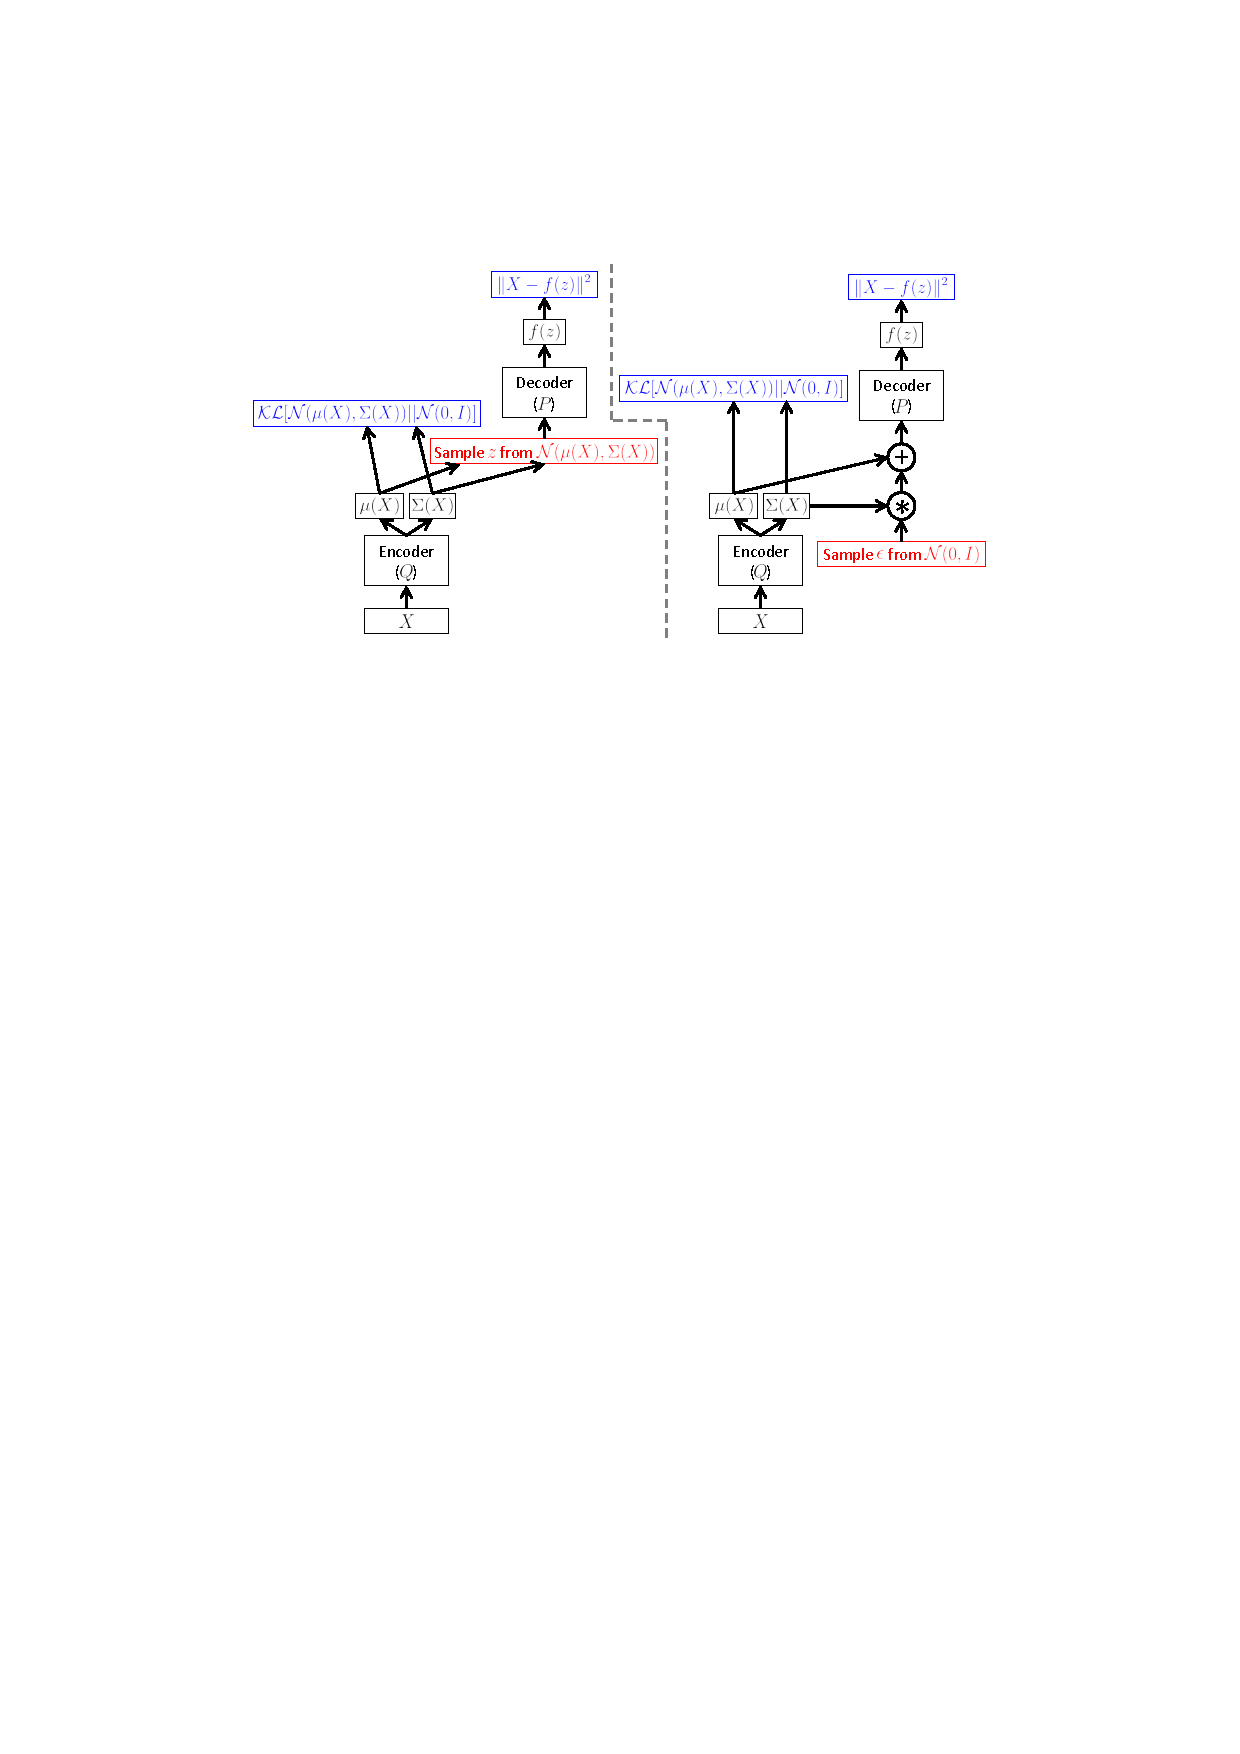
\includegraphics[width=\textwidth]{vae2.pdf}

\blfootnote{From Carl Doersch's Tutorial on VAEs - https://arxiv.org/pdf/1606.05908.pdf}
\end{frame}

%-------------------------------------------------------------%

\begin{frame}
\frametitle{VAE Models and Performance}

\begin{itemize}
  \item<+-> VAEs can be used with any kind of data
  \begin{itemize}
    \item the distributions and network architecture just needs to be set accordingly
    \item e.g. it's common to use convolutions in the encoder and transpose convolutions in (Gaussian) decoder for image data
  \end{itemize}
  \item<+-> VAEs have nice learning dynamics; they tend to be easy to optimise with stable convergence
  \item<+-> VAEs have a reputation for producing blurry reconstructions of images
  \begin{itemize}
    \item Not fully understood why, but most likely related to a side effect of maximum-likelihood training
  \end{itemize}
  \item<+-> VAEs tend to only utilise a small subset of the dimensions of $\bm z$
  \begin{itemize}
    \item Pro: automatic latent variable selection
    \item Con: better reconstructions should be possible given the available code-space
  \end{itemize}
\end{itemize}

\end{frame}

\begin{frame}
\frametitle{Reconstructions Example}
\begin{center}
  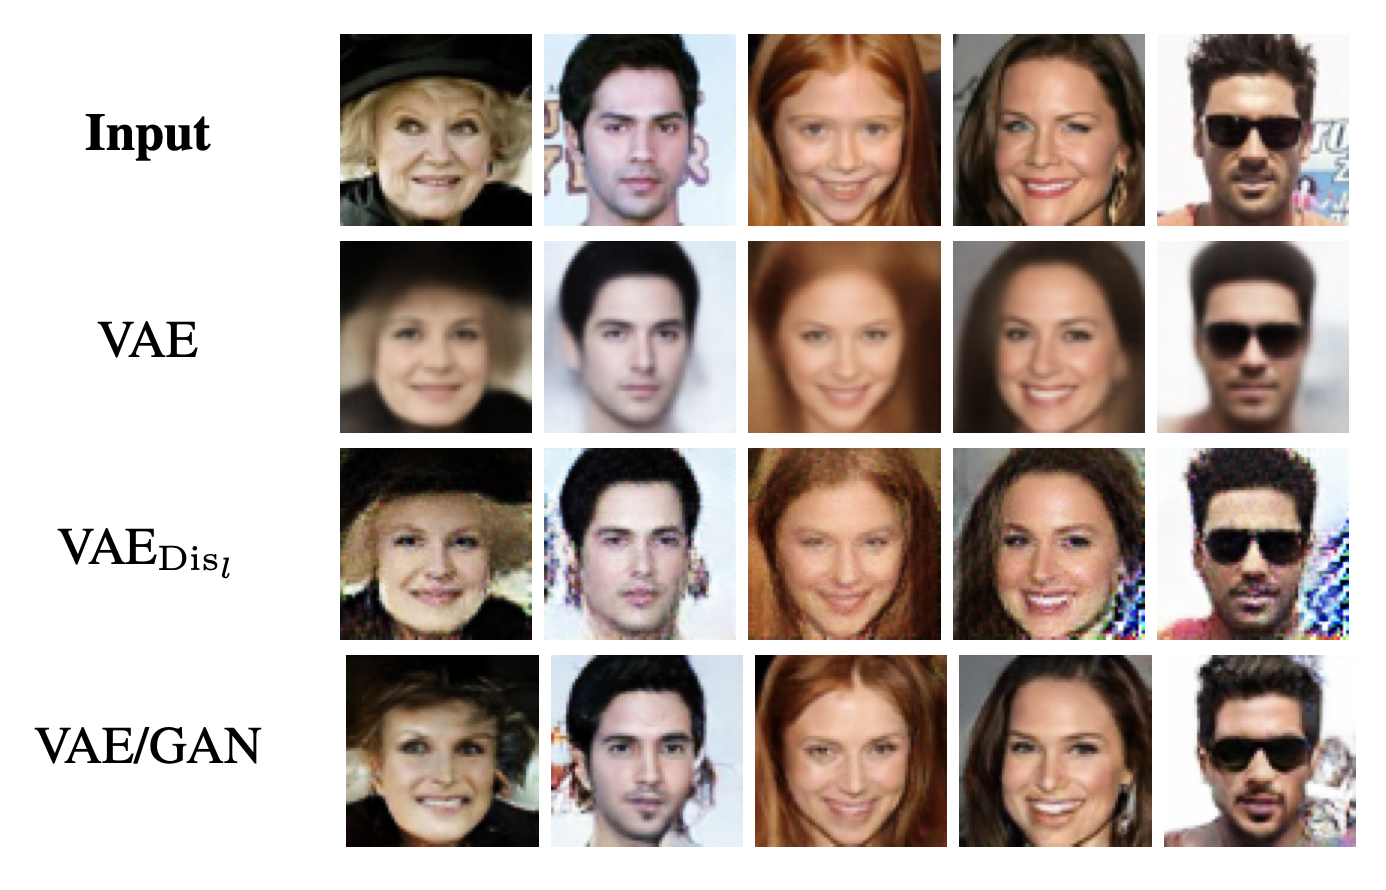
\includegraphics[width=\textwidth]{vaegan.png}
\end{center}
\end{frame}
%-------------------------------------------------------------%

\begin{frame}
\frametitle{Sampling Example}
\begin{center}
  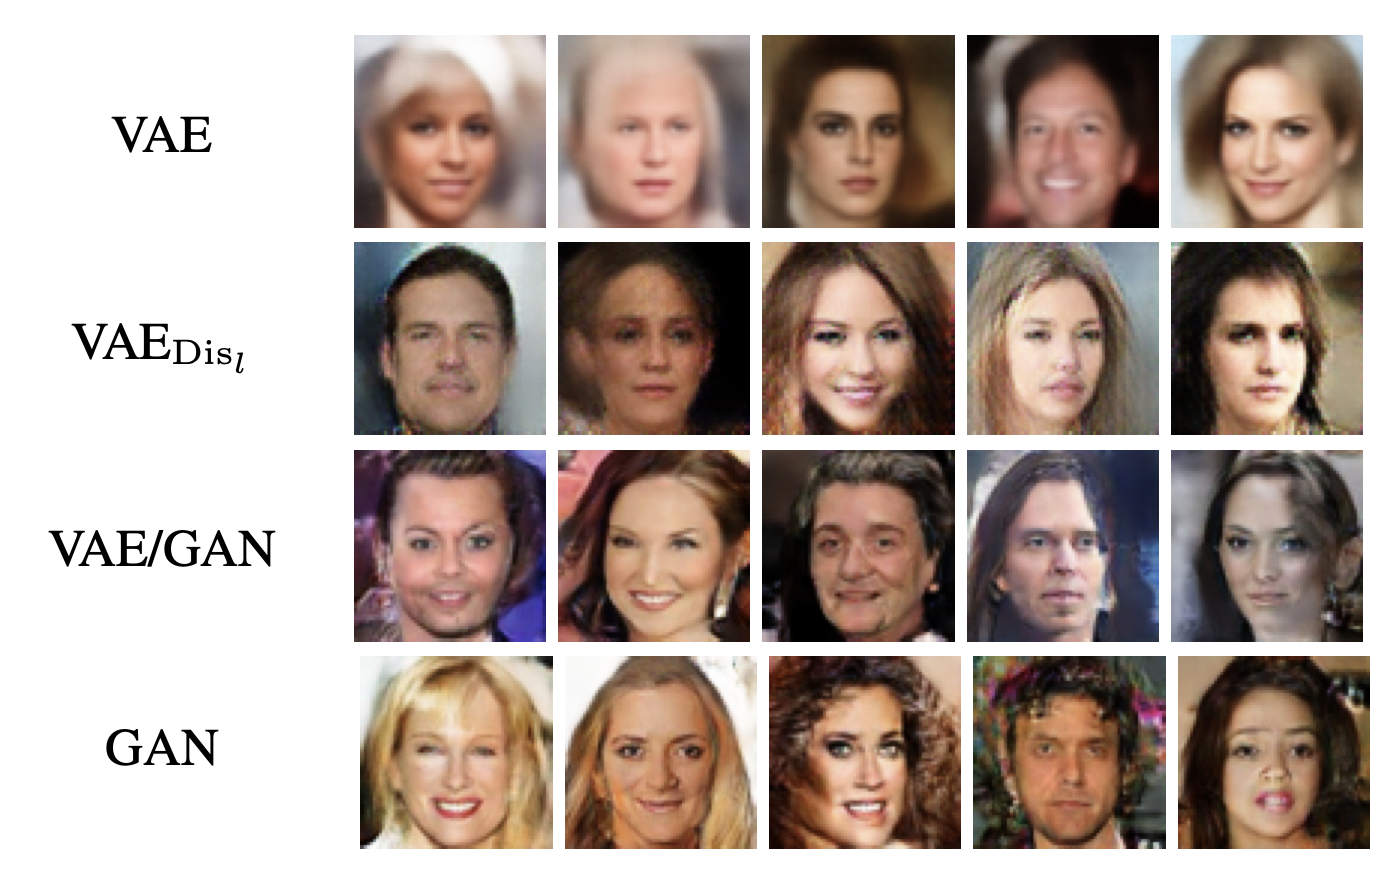
\includegraphics[width=\textwidth]{vaegan-samples.png}
\end{center}
\end{frame}
%-------------------------------------------------------------%
\section{Generative Adversarial Networks}

\begin{frame}
\frametitle{Generative Adversarial Networks (GANs)}
\begin{itemize}
\item<+-> New (old?!\footnote{c.f. Schmidhuber}) method of training deep generative models 
\item<+-> Idea: pitch a generator and a discriminator against each other 
\begin{itemize}
\item Generator tries to draw samples from $p(\mathrm{x})$ 
\item Discriminator tries to tell if sample came from the generator (fake) or the real world 
\end{itemize}
\item<+-> Both discriminator and generator are deep networks (differentiable functions) 
\item<+-> LeCun quote `GANs, the most interesting idea in the last ten years in machine learning'
\end{itemize}
\end{frame}
%-------------------------------------------------------------%

\begin{frame}[fragile]\frametitle{Aside: Adversarial Learning vs. Adversarial Examples}
The approach of GANs is called adversarial since the two networks have \emph{antagonistic} objectives.\\ \vspace{0.5cm}

This is not to be confused with \emph{adversarial examples} in machine learning. \vspace{0.5cm}

See these two papers for more details: \\
\url{https://arxiv.org/pdf/1412.6572.pdf} \\
\url{https://arxiv.org/pdf/1312.6199.pdf}
\end{frame}
%-------------------------------------------------------------%

\begin{frame}[fragile]
\begin{figure}
\center  
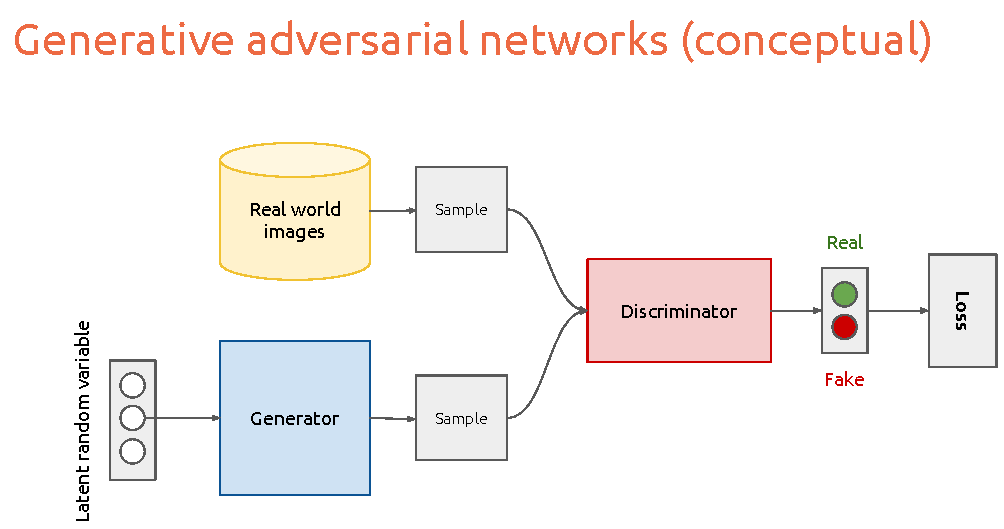
\includegraphics[width=\textwidth]{figs/GANS_1.pdf} \blfootnote{Picture Credit: Xavier Giro-i-Nieto}
\end{figure}
\end{frame}
%-------------------------------------------------------------%

\begin{frame}[fragile]{pause}\frametitle{More Formally}
\begin{itemize}
\item The {\bf generator}
		\begin{equation*}
		\bm x = g(\bm z)
		\end{equation*}
		
		is trained so that it gets a random input $\bm z \in \mathbb{R}^n$ from a distribution (typically $\mathcal{N}(\bm 0, \bm I)$ or $\mathcal{U}(\bm 0, \bm I)$) and produces a sample $\bm x \in \mathbb{R}^d$ following the data distribution as output (ideally). Usually $n<<d$. \vspace{1cm}

\item The {\bf discriminator}
	\begin{equation*}
	y = d(\bm x)
	\end{equation*}
	gets a sample $\bm x$ as input and predicts a probability $y \in [0, 1]$ (or real-valued logit of a Bernoulli distribution) determining if it is real or fake.
\end{itemize}
\end{frame}
%-------------------------------------------------------------%

\begin{frame}
\frametitle{More Practically}

\begin{itemize}
  \item Training a standard GAN is difficult and often results in two undesirable behaviours
  \begin{itemize}
    \item Oscillations without convergence. No guarantee that the loss will actually decrease...
    \begin{itemize}
      \item It has been shown that a GAN has saddle-point solution, rather than a local minima.
    \end{itemize}
  \item The {\bf mode collapse} problem, when the generator models very well a small sub-population, concentrating on a few modes.
  \end{itemize}
  \item Additionally, performance is hard to assess and often boils down to heuristic observations.
\end{itemize}
\end{frame}

%-------------------------------------------------------------%

\begin{frame}
\frametitle{Deep Convolutional Generative Adversarial Networks (DCGANs)}

\begin{columns}
\begin{column}{0.45\textwidth}
\begin{itemize}
\item Motivates the use of GANS to learn reusable feature representations from large unlabelled datasets.
\item GANs known to be unstable to train, often resulting in generators that produce ``nonsensical outputs''.
\item Model exploration to identify architectures that result in {\bf stable} training across datasets with higher resolution and deeper models. 
\end{itemize}
\end{column}
\begin{column}{0.55\textwidth}
  \begin{figure}
    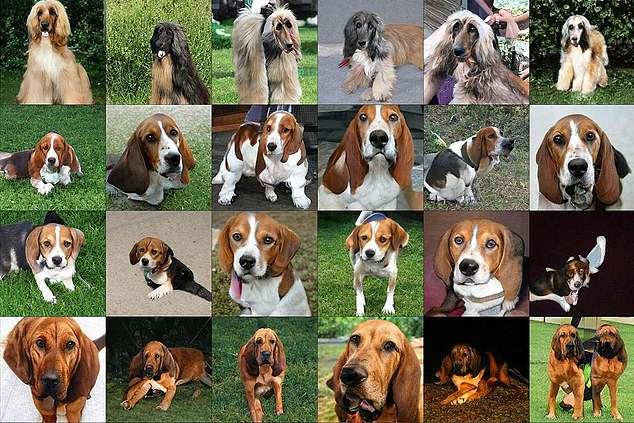
\includegraphics[width=\columnwidth]{dogs.jpg}
  \end{figure}
\end{column}
\end{columns}
\end{frame}

%-------------------------------------------------------------%

\begin{frame}
\frametitle{Architecture Guidelines for Stable DCGAN}

\begin{itemize}
\item<+-> Replace pooling layers with strided convolutions in the discriminator and fractional-strided (transpose) convolutions in the generator.  
\begin{itemize}
  \item This will allow the network to learn its own spatial downsampling. 
\end{itemize}
\item<+-> Use batchnorm in both the generator and the discriminator. 
\begin{itemize}
  \item This helps deal with training problems due to poor initialisation and helps the gradient flow. 
\end{itemize}
\item<+-> Eliminate fully connected hidden layers for deeper architectures. 
\item<+-> Use ReLU activation in the generator for all layers except for the output, which uses $\tanh$. 
\item<+-> Use LeakyReLU activation in the discriminator for all layers.
\end{itemize}
\end{frame}
%-------------------------------------------------------------%

\begin{frame}
\frametitle{Summary}

\begin{itemize}
  \item Generative modelling is a massive field with a long history
  \item Differentiable generators have had a profound impact in making models that work with real data at scale
  \item VAEs and GANs are currently the most popular approaches to training generators for spatial data
  \item We've only scratched the surface of generative modelling
  \begin{itemize}
    \item Auto-regressive approaches are popular for sequences (e.g. language modelling). 
      \begin{itemize}
        \item But also for images (e.g. PixelRNN, PixelCNN)
      \end{itemize}
      \item typically RNN-based
      \item but not necessarily - e.g. WaveNet is a convolutional auto-regressive generative model
  \end{itemize}
\end{itemize}
\end{frame}

\end{document}